\documentclass[tikz]{standalone}
\usepackage{tikz} 
\usetikzlibrary{shapes.misc,patterns,hobby}
\usepackage{pgfplots}
\usepgfplotslibrary{fillbetween}
%\usepackage[active,tightpage]{preview}  %generates a tightly fitting border around the work
%\PreviewEnvironment{tikzpicture}
%\setlength\PreviewBorder{2mm}
\usepackage{xcolor}
\definecolor{myred}{RGB}{196,19,47} 
\definecolor{myblue}{RGB}{0,139,139}

\begin{document}
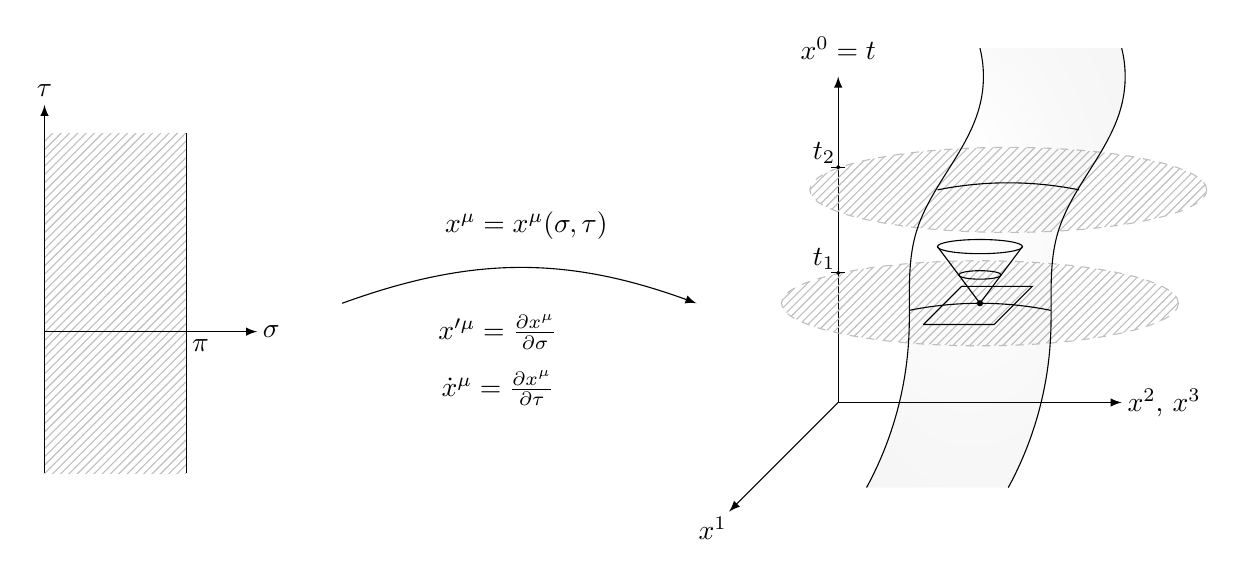
\begin{tikzpicture}[xscale=1.8,yscale=1.8,>=latex]
%Füllung des Rechtecks mit Strichen ( zuerst damit die schwarzen Linien drüberliegen)
\path[pattern=north east lines, pattern color=gray!50] plot coordinates {(0.4,-1) (1.4,-1) (1.4,1.4) (0.4,1.4)}; 

%Koordinatensystem links mit Beschriftung 
\draw[->, thin] (0.4,-1) to (0.4,1.6);
\node at (0.4,1.7) {$\tau$};
\draw[->, thin] (0.4,0) to (1.9,0);
\node at (2,0) {$\sigma$};
\draw[-, thin] (1.4,-1) to (1.4,1.4);
\node at (1.5,-0.1) {$\pi$};
  
 
%Verbindungslinie mit Formeln
\draw[thin,->] (2.5,0.2) [out=20, in=160] to (5,0.2);
\node at (3.8,0.75) {$x^{\mu} = x^{\mu}(\sigma,\tau)$};
\node at (3.6,0) {$x'^{\mu} = \frac{\partial x^{\mu}}{\partial \sigma}$};
\node at (3.6,-0.4) {$\dot{x}^{\mu} = \frac{\partial x^{\mu}}{\partial \tau}$};  

%Koordinatensystem rechts (3D)
\draw[->, thin] (6,-0.5,0) to (6,-0.5,2);
\node at (6,-0.5,2.3) {$x^1$};
\draw[->, thin] (6,-0.5,0) to (8,-0.5,0);
\node at (8.3,-0.5,0) {$x^2$, $x^3$};
\draw[->, thin] (6,-0.5,0) to (6,1.8,0);
\node at (6,2,0) {$x^0 = t$};
  
%gefüllte Kreisebene unten 
\path[pattern=north east lines, pattern color=gray!50] (7,0.2) ellipse (1.4 and 0.3); 
\path[draw, dashed,color=gray!50] (7,0.2) ellipse (1.4 and 0.3); 
\filldraw (6,0.415,0) circle (0.3pt);
\draw[-, thin] (5.95,0.415) to (6.05,0.415);
\node at (5.9,0.51,0) {$t_1$};
%gefüllte Kreisebene oben
\path[pattern=north east lines, pattern color=gray!50] (7.2,1) ellipse (1.4 and 0.3); 
\path[draw, dashed,color=gray!50] (7.2,1) ellipse (1.4 and 0.3); 
\filldraw (6,1.16,0) circle (0.3pt);
\draw[-, thin] (5.95,1.16) to (6.05,1.16);
\node at (5.9,1.26,0) {$t_2$};


\newcommand\kurve{(6.2,-1.1) to [curve through = { (6.5,0) (6.55,0.7) (7,1.6)  }] (7,2)}
\newcommand\kurvee{(8,2) to [curve through = { (8,1.6) (7.55,0.7) (7.5,0) }] (7.2,-1.1)}

\def\mypath{\kurve -- \kurvee -- (6.2,-1.1)}

\draw[-] \kurve;
\draw[-] \kurvee;

\shade[ball color = gray!30, opacity = 0.05] \mypath;


%Verbindungen
\draw[-] (6.5,0.15) to [curve through = { (7,0.2)  }] (7.5,0.15);
\draw[-] (6.7,1) to [curve through = { (7.2,1.05)  }] (7.7,1);

%Quadrat unten
\path[draw, color = black, thin] (6.6,0.05,0) to (7.1,0.05,0) to (7.1,0.05,-0.7) to (6.6,0.05,-0.7) to (6.6,0.05,0);

%Kegel
\filldraw (7,0.2) circle (0.5pt);
\draw[-,thin] (7,0.2) to (6.7,0.6);
\draw[-,thin] (7,0.2) to (7.3,0.6);
\draw (7,0.6) ellipse (0.3 and 0.05);

%innerer Kreis mit Massenpunkt
\draw (7,0.4) ellipse (0.15 and 0.03);



\end{tikzpicture}
\end{document}